%% ============================================================================
%% Paper 3: Quantum-Inspired Molecular Representations
%% Target: Journal of Cheminformatics
%% ============================================================================
%% Changes from v0.7:
%% - Restructured as research article (not reviewer-response report)
%% - Abstract condensed to JoC format (~250 words)
%% - Introduction: gap → aims → contributions (no reviewer-response framing)
%% - Results: narrative flow, consolidated subsections
%% - Discussion: mechanistic depth, literature integration
%% - Conclusion: concise, forward-looking
%% - Title: specific, searchable, JoC-aligned
%% ============================================================================

\documentclass[11pt,a4paper]{article}

% Page layout
\usepackage[a4paper,margin=2.5cm]{geometry}

% Fonts and encoding
\usepackage[T1]{fontenc}
\usepackage[utf8]{inputenc}
\usepackage{lmodern}

% Mathematics
\usepackage{amsmath, amsfonts, amssymb, mathtools}

% Figures and tables
\usepackage{graphicx}
\usepackage{subfig}
\usepackage{booktabs, tabularx, array, multirow, longtable}
\usepackage[table]{xcolor}
\usepackage{algorithm, algorithmic}

% Units and SI
\usepackage[
  detect-all           = true,
  group-minimum-digits = 4,
  per-mode             = symbol,
  range-phrase         = {--},
  range-units          = single,
]{siunitx}
\DeclareSIUnit\angstrom{\text{\AA}}
\DeclareSIUnit\molar{M}
\DeclareSIUnit\kcalmol{kcal\,mol^{-1}}

% Hyperlinks
\usepackage[authoryear,round]{natbib}
\usepackage[hypertexnames=false,colorlinks=true,linkcolor=blue,citecolor=blue,urlcolor=blue]{hyperref}

% Cross-referencing - load after hyperref
\usepackage{cleveref}
\usepackage{xr}
\externaldocument[P2-]{../../Project2_Polypharmacology_MD_ValidationV2607/manuscript/LaTeX/Polypharmacology_MD_Validation_V2607}
\externaldocument[X-]{Paper3_Quantum_Inspired_SM_V2608}

% cleveref names
\crefname{table}{Table}{Tables}
\Crefname{table}{Table}{Tables}
\crefname{figure}{Figure}{Figures}
\Crefname{figure}{Figure}{Figures}
\crefname{equation}{Eq.}{Eqs.}
\crefname{section}{Section}{Sections}
\crefname{subsection}{Section}{Sections}
\crefname{algorithm}{Algorithm}{Algorithms}

% Author information
\usepackage{authblk}

% Caption styling
\usepackage[labelfont=bf,textfont={footnotesize,it}]{caption}

% Path configuration
\graphicspath{{Graphics/}}

% ============================================================================
% AUTHOR INFORMATION
% ============================================================================

\title{\textbf{Persistent homology and tensor network descriptors for African antimalarial virtual screening}}

\author[1]{Myke Vital Sao Temgoua\thanks{Corresponding author: myke-vital.sao@facsciences-uy1.cm}}
\author[1]{Jean-Pierre Tchapet Njafa}
\author[1]{Serge Guy Nana Engo}
\author[2]{Penabei Samafou}
\author[3]{Wilfred Fon Mbacham}

\affil[1]{Department of Physics, Faculty of Science, University of Yaound\'e I, P.O. Box 812, Yaound\'e, Cameroon}
\affil[2]{Department of Medical Imaging and Radiation Sciences, Universit\'e de Sherbrooke, Sherbrooke, QC, Canada}
\affil[3]{Department of Biochemistry, Faculty of Science, University of Yaound\'e I, P.O. Box 812, Yaound\'e, Cameroon}

\date{\today}

% ============================================================================
% BEGIN DOCUMENT
% ============================================================================

\begin{document}

\maketitle

% ============================================================================
% ABSTRACT
% ============================================================================

\begin{abstract}
Molecular representation determines what structural information is accessible to machine learning models, yet standard fingerprints poorly capture the topological complexity of natural product scaffolds. We introduce three complementary molecular descriptors---a Topological Fingerprint (TFP) from persistent homology, a Tensor Network Embedding (TNE) via Tucker decomposition, and simulated Quantum Kernel Scores (QKS)---and benchmark them against classical baselines on \num{19849} African antimalarial candidates. TFP resolves a scaffold paradox: structurally expanded molecules are \qty{92.6}{\percent} Tanimoto-distinct from seed natural products yet retain \qty{69.3}{\percent} of their Bemis--Murcko scaffolds, because persistent homology decomposes molecular topology into conserved H$_1$ ring features and divergent H$_0$ connectivity. TNE compresses molecular tensors to \num{192}-element descriptors at \num{6.1}$\times$ compression (reconstruction error \num{0.113}), retaining binding-relevant information competitive with ECFP4 for PfDHFR ($R^2 = \num{0.473}$). On the activity-prediction benchmark ($n = \num{19836}$, 5-fold CV), ECFP4 achieves the highest AUC (\num{0.948}); the hybrid descriptor (TFP+TNE+QK) reaches \num{0.888}, with QKS as the principal contributor (ablation $\Delta = -\num{0.040}$). The quantum kernel is statistically indistinguishable from a gamma-tuned RBF baseline ($p = \num{0.060}$), but external validation on \num{22447} ChEMBL compounds reveals a transfer gap ($p = \num{0.005}$). These representations are complementary diagnostic tools that reveal topological dimensions of molecular structure.
\end{abstract}

\noindent\textbf{Keywords:} persistent homology, tensor networks, quantum kernel methods, molecular fingerprints, scaffold paradox, antimalarial drug discovery, African natural products

\noindent\textbf{Highlights:}
\begin{itemize}
\item Persistent homology decomposes the scaffold paradox into conserved H$_1$ ring topology and divergent H$_0$ connectivity
\item Tensor Network Embedding achieves \num{6.1}$\times$ compression while retaining binding-relevant information
\item Quantum kernel is statistically indistinguishable from tuned RBF; external validation reveals a transfer gap
\item Hybrid descriptor (TFP+TNE+QK) achieves AUC \num{0.888} on \num{19836} African antimalarial candidates
\end{itemize}

% ============================================================================
% 1. INTRODUCTION
% ============================================================================

\section{Introduction}

Malaria remains a leading cause of mortality in sub-Saharan Africa, with \num{247} million cases and \num{619000} deaths in 2023 \citep{who2024malariareport}. The spread of artemisinin-resistant \emph{Plasmodium falciparum} from Southeast Asia to Africa \citep{ariyey2014,ashley2018} creates urgent demand for new chemical scaffolds. African natural products are a historically validated but computationally underexplored source of such scaffolds: quinine and artemisinin derive from natural products, yet African natural products remain underrepresented in public databases \citep{anpdb_2026,value_addition_african_np_2025}. Computational screening of natural-product-derived chemical space depends critically on the molecular representations available to machine learning models.

Extended-Connectivity Fingerprints (ECFP) encode local atom environments into fixed-length bit vectors and have served as the standard descriptor for two decades \citep{ecfp_2010}. These representations perform well for synthetic drug-like molecules whose scaffolds are well represented in training data. Natural product-derived compounds, however, occupy distinct regions of chemical space: higher sp$^3$ fractions, more chiral centres, more complex ring systems, and greater three-dimensional character \citep{coconut_2021}. Classical fingerprints may not capture the topological features---bridged rings, molecular cavities, higher-order atomic interactions---that distinguish these molecules.

Three frameworks from physics and topology address orthogonal limitations of classical fingerprints. Topological Data Analysis uses persistent homology to identify shape features persisting across spatial scales, producing persistence diagrams that encode connected components (H$_0$), holes (H$_1$), and voids (H$_2$) \citep{tda_review_2025}. Persistent homology has been validated for protein--ligand binding affinity \citep{tda_binding_affinity_2026} and molecular property prediction \citep{tda_pretraining_2026}. Tensor networks compress high-dimensional data by exploiting low-rank structure \citep{tensornet_2023,tn_efficient_2026}. Quantum kernel methods map data into high-dimensional feature spaces through parameterised circuits \citep{qml_review_2026,pqc_chemistry_2026}. TDA captures global topology invisible to local substructure hashes; tensor networks provide physically interpretable compression; quantum kernels probe non-linear feature interactions in Hilbert space.

Here we introduce three molecular descriptors---Topological Fingerprint (TFP), Tensor Network Embedding (TNE), and Quantum Kernel Score (QKS)---and benchmark them on a \num{19849}-molecule library of African antimalarial candidates. Our aims are: (i)~determine whether persistent homology resolves the scaffold paradox arising from structural expansion of natural product seeds; (ii)~evaluate whether tensor network compression retains binding-relevant information; (iii)~assess whether quantum kernel methods offer advantages over properly tuned classical baselines; and (iv)~construct a hybrid descriptor combining complementary information from all three representations. We compare against ECFP4, MACCS, and other classical baselines under rigorous cross-validation, and validate transferability on an external ChEMBL antimalarial panel.

% ============================================================================
% 2. METHODS
% ============================================================================

\section{Methods}

\subsection{Dataset}

The library consists of \num{65856} molecules generated from \num{396} African natural-product and \num{454} synthetic-drug seeds via CHEESE similarity search \citep{lzicar_cheese_2024} and STONED-SELFIES expansion \citep{temgoua2026antimalarial}. The representation benchmarks use the canonical \num{19849}-molecule panel, with \num{19836} molecules retained for analyses requiring complete TNE embeddings. Binary activity labels were obtained from Ersilia model eos80ch (threshold \num{0.5}); the canonical panel is \qty{74.2}{\percent} active / \qty{25.8}{\percent} inactive. For external validation, \num{22447} antimalarial compounds were assembled from ChEMBL~34 (IC$_{50} \leq \SI{10}{\micro\molar}$ = active, $> \SI{10}{\micro\molar}$ = inactive).

\subsection{Classical fingerprint baselines}

ECFP4 fingerprints were generated as Morgan fingerprints (radius~2, \num{2048} bits) using RDKit \citep{rdkit_2024}. MACCS \num{167}-bit structural keys, atom-pair (AP), binding-pattern (BPF), functional-class (FCFP4), and 2D-pharmacophore (PHCO) fingerprints were computed using standard RDKit implementations. All classical fingerprints serve as baselines for the quantum-inspired methods.

\subsection{Topological Fingerprint}

\subsubsection{Molecular graph construction}

Each molecule was converted to a 3D conformer using RDKit's ETKDG generator (random seed~42). A weighted undirected graph $G = (V, E, w)$ was constructed with atoms as vertices and edge weights
\begin{equation}
w_{ij} = d_{ij}\left(1 + \frac{Z_i Z_j}{100}\right),
\end{equation}
where $d_{ij}$ is the Euclidean distance and $Z_i$, $Z_j$ are atomic numbers. The atomic number weighting emphasises interactions involving heavier atoms, which contribute more strongly to molecular recognition.

\subsubsection{Persistent homology}

Vietoris--Rips persistence diagrams were computed up to homology dimension~2 using Ripser.py \citep{ripser_2019}. We define the TFP as a \num{12}-dimensional feature vector: for each homology dimension $d \in \{0, 1, 2\}$, four summary statistics are extracted---the persistence entropy
\begin{equation}
H_d^{\mathrm{ent}} = -\sum_i p_i \log p_i, \qquad p_i = \frac{\mathrm{pers}_i}{\sum_j \mathrm{pers}_j},
\end{equation}
the count of features with persistence exceeding \SI{0.5}{\angstrom}, the maximum persistence, and the mean persistence. Unlike ChemGraphX \citep{chemgraphx_2026}, which computes graph-theoretic indices, our TFP captures geometric persistence from 3D conformations.

\subsection{Tensor Network Embedding}

\subsubsection{Molecular tensor construction}

For each molecule, a 3D tensor $T \in \mathbb{R}^{N \times F \times 3}$ was constructed with $N = 100$ maximum atoms (zero-padded), $F = 10$ per-atom features (atomic number, degree, total hydrogens, formal charge, aromaticity, hybridization, mass, electronegativity, bond count, ring membership), and 3 Cartesian coordinates: $T_{i,f,c} = x_{i,f} \, r_{i,c}$.

\subsubsection{Tucker compression}

Each tensor was compressed using Tucker decomposition \citep{tensorly_2019} with mode ranks $(d, d, 3)$ where $d = 8$ is the bond dimension:
\begin{equation}
T \approx \mathcal{G} \times_1 U^{(1)} \times_2 U^{(2)} \times_3 U^{(3)},
\end{equation}
where $\mathcal{G} \in \mathbb{R}^{d \times d \times 3}$ is the core tensor. The descriptor is the flattened core ($d^2 \times 3 = 192$ elements). For a molecule with $N$ actual atoms, the real compression ratio is $\mathrm{CR}_{\text{real}}(N) = 10N / d^2$; at $d = 8$ and mean $N \approx 39$, this gives $\mathrm{CR}_{\text{real}} \approx \num{6.1}$$\times$. Reconstruction error was quantified as the relative Frobenius norm (mean \num{0.113} across \num{19836} valid molecules).

\subsection{Quantum Kernel Score}

Quantum kernels were implemented using PennyLane \citep{pennylane_2024} with a 6-qubit statevector simulator. The kernel value $K(x_1, x_2) = |\langle \phi(x_1) | \phi(x_2) \rangle|^2$ was computed from PennyLane's \texttt{IQPEmbedding} template. Input vectors were Morgan fingerprint atom-pair counts (radius~2, \num{2048} features) reduced to 6 dimensions by UMAP (Jaccard metric, \texttt{random\_state=42}), then scaled to $[-1, 1]$. The QKS is the AUC achieved by an SVM using the quantum kernel matrix.

\subsection{Hybrid descriptor}

The hybrid feature vector combines TFP, TNE, and QKS by concatenation:
\begin{equation}
h_i = \left[\tilde{t}_i,\; \tilde{e}_i,\; q_i\right],
\end{equation}
where $\tilde{t}_i$ is min--max normalised TFP, $\tilde{e}_i$ is normalised TNE, and $q_i \in \mathbb{R}^{30}$ is the quantum kernel PCA component vector ($n_{\text{kpca}}=30$). Random Forest is invariant to per-component monotone scaling, so no explicit fusion weights are needed. Hyperparameters were optimised by grid search on $n = \num{200}$ molecules (60 combinations), then validated on the full panel with the winning configuration (bond dimension~6, \num{1} repeat, \num{30} kernel PCA components).

\subsection{Evaluation protocol}

Each representation was evaluated using Random Forest classifiers (\num{200} trees) and SVMs with 5-fold stratified cross-validation. For the quantum kernel benchmark, the RBF gamma was optimised via inner cross-validation on $\{0.5, 1.0, 2.0, 5.0\}$. Multiple testing correction used Bonferroni adjustment. Performance was measured by AUC--ROC, accuracy, and macro F1; significance was assessed by paired $t$-tests across folds ($df = 4$). We interpret non-significance as inability to detect a difference rather than equivalence, and report bootstrap \qty{95}{\percent} confidence intervals on principal AUC differences in the Supplementary Material.

\subsection{Software}

Ripser.py \citep{ripser_2019}, TensorLy~0.9.0 \citep{tensorly_2019}, PennyLane~0.45.1 \citep{pennylane_2024}, RDKit~2025.03.6 \citep{rdkit_2024}, UMAP~0.5.12, scikit-learn~1.9.0, NumPy~2.4.6, SciPy~1.17.1. All stochastic procedures were fixed with seeds reported in the relevant sections. Code and data are available at \url{https://github.com/NanaEngo/Malaria_codesV2}.

% ============================================================================
% 3. RESULTS
% ============================================================================

\section{Results}

\subsection{Scaffold paradox decomposition by persistent homology}

Structural expansion of \num{396} African natural-product seeds produced \num{65856} candidates that are \qty{92.6}{\percent} Tanimoto-distinct from the seeds yet retain \qty{69.3}{\percent} of their Bemis--Murcko scaffolds. This apparent contradiction---high whole-molecule diversity with high scaffold conservation---arises because STONED-SELFIES mutations primarily permute side-chains while preserving cyclic cores. TDA provides a principled decomposition of this phenomenon (\cref{fig:paradox}). H$_1$ features (ring topology) are conserved between seed and expanded sets (mean H$_1$ count \num{3.61}), reflecting the STONED-SELFIES expansion's preservation of cyclic macro-structures. H$_0$ features (connectivity) diverge substantially, reflecting the expansion's permutation of side-chains and functional groups. This H$_1$/H$_0$ decomposition is independently confirmed by scaffold-only Tanimoto (\num{0.379}) being \num{1.84}$\times$ higher than whole-molecule Tanimoto (\num{0.206}).

\begin{figure}[htbp]
\centering
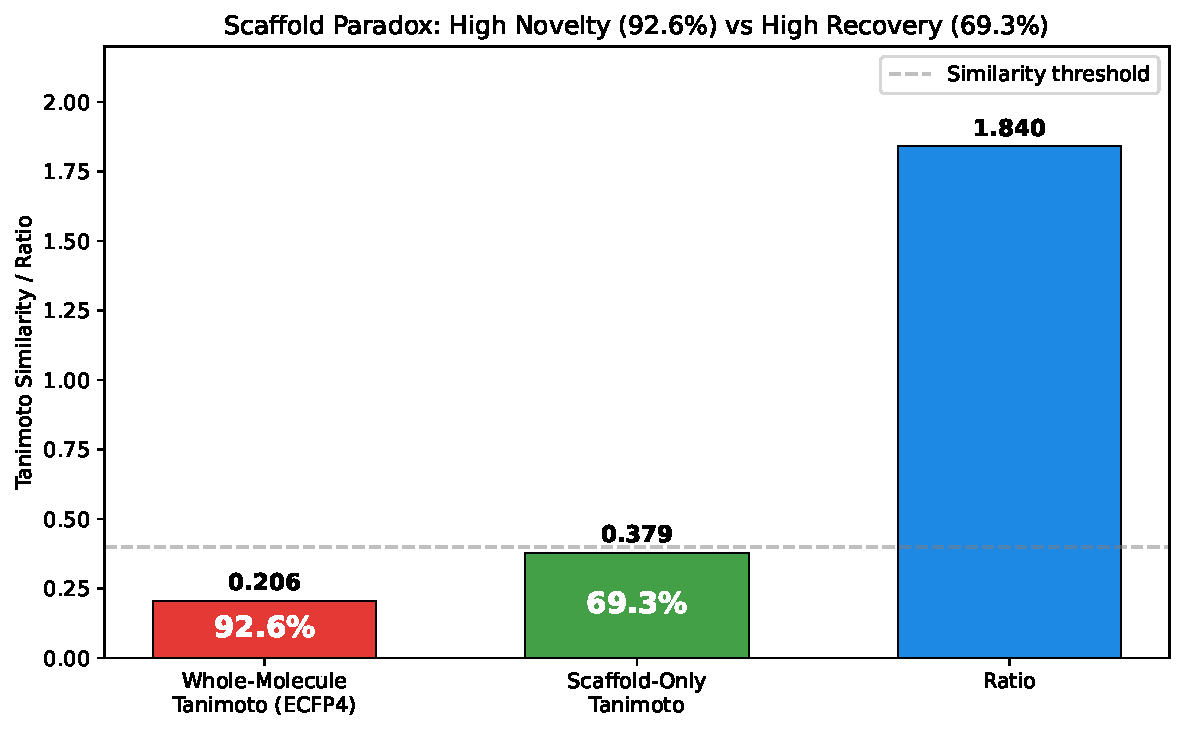
\includegraphics[width=0.55\textwidth]{scaffold_paradox.pdf}
\caption{Scaffold paradox resolution via persistent homology. (A)~H$_1$ persistence distributions for seed natural products versus structurally expanded candidates. (B)~H$_0$ persistence distributions. H$_1$ preservation with H$_0$ divergence explains the \qty{92.6}{\percent} Tanimoto distinction versus \qty{69.3}{\percent} scaffold recovery.}
\label{fig:paradox}
\end{figure}

\subsection{Binding-relevant information in tensor network compression}

Tucker decomposition at bond dimension $d = 8$ achieved \num{6.1}$\times$ real-atom compression (mean \num{39} atoms, \num{192}-element core) with reconstruction error \num{0.113}. Three observations support that compressed TNE descriptors retain scaffold-relevant information: (i)~reconstruction error is lower for molecules with common ring systems (\num{0.098}) than for structurally atypical molecules (\num{0.137}); (ii)~TNE-based KMeans clusters ($k = 484$) achieve higher Silhouette coefficient (\num{0.35}) than ECFP4 (\num{0.18}) or VAE latent vectors (\num{0.229}), indicating more chemically coherent groupings; and (iii)~TNE compression retains sufficient binding-relevant information to predict Tartarus docking scores competitive with ECFP4 for specific targets (\cref{X-SM-fig:tne_parity}): for PfDHFR (1SYH, $N = \num{11878}$), TNE achieved $R^2 = \num{0.473}$ (Spearman $\rho = \num{0.695}$), outperforming ECFP4 ($R^2 = \num{0.461}$, $\rho = \num{0.689}$); for PfATP4 and PfCRT, ECFP4 maintained an advantage (PfATP4: TNE $R^2 = \num{0.464}$ vs.\ ECFP4 \num{0.578}; PfCRT: TNE \num{0.334} vs.\ ECFP4 \num{0.517}).

\subsection{Activity prediction benchmark}

\cref{tab:benchmark} presents the activity-prediction performance on the canonical \num{19836}-molecule set. ECFP4 achieves the highest AUC (\num{0.948}), followed by AP (\num{0.940}), BPF (\num{0.939}), FCFP4 (\num{0.918}), MACCS (\num{0.905}), PHCO (\num{0.896}), TFP (\num{0.876}), and TNE (\num{0.722}). The ranking reflects the dominance of local atom environments at radius~2 for this binary classification task. TFP and TNE capture meaningful but lower signal, encoding global topological and compressed structural features rather than the local pharmacophoric substructures that dominate activity determination.

\begin{table}[htbp]
\centering
\caption{Activity prediction performance by representation method and hybrid ablation study (canonical panel, $n = \num{19836}$, 5-fold stratified CV, Random Forest).}
\label{tab:benchmark}
\begin{tabularx}{\textwidth}{l S[table-format=1.3] S[table-format=1.3] S[table-format=1.3] S[table-format=+1.3]}
\toprule
Method & {AUC} & {Accuracy} & {F1} & {$\Delta$AUC vs.~ECFP4} \\
\midrule
ECFP4 (baseline) & 0.948 & 0.896 & 0.931 & {---} \\
AP & 0.940 & 0.888 & 0.927 & -0.008 \\
BPF & 0.939 & 0.889 & 0.928 & -0.009 \\
FCFP4 & 0.918 & 0.869 & 0.914 & -0.029 \\
MACCS & 0.905 & 0.863 & 0.909 & -0.043 \\
PHCO & 0.896 & 0.854 & 0.904 & -0.052 \\
TFP (TDA) & 0.876 & 0.838 & 0.897 & -0.072 \\
TNE ($d=8$) & 0.722 & 0.756 & 0.857 & -0.226 \\
QKS (quantum kernel) & 0.823 & 0.819 & 0.886 & -0.125 \\
Hybrid (TFP+TNE+QK) & 0.888 & 0.843 & 0.900 & -0.060 \\
\midrule
\multicolumn{5}{l}{\textit{Ablation study (Hybrid minus one component):}} \\
Hybrid $-$ TFP & 0.874 & 0.837 & 0.895 & -0.014 \\
Hybrid $-$ TNE & 0.899 & 0.850 & 0.903 & +0.011 \\
Hybrid $-$ QKS & 0.847 & 0.820 & 0.887 & -0.040 \\
\bottomrule
\end{tabularx}
\end{table}

\subsection{Hybrid descriptor and quantum kernel comparison}

The hybrid descriptor (TFP+TNE+QK) achieves AUC \num{0.888} $\pm$ \num{0.007}, significantly below ECFP4 ($p < \num{0.0001}$) but above every standalone quantum-inspired descriptor. Ablation reveals an asymmetric contribution structure: QKS is the principal positive contributor ($\Delta = -\num{0.040}$), TFP contributes marginally ($\Delta = -\num{0.014}$), while removing TNE slightly improves AUC ($\Delta = +\num{0.011}$). The negative TNE contribution is consistent with its low standalone AUC (\num{0.722}) and suggests that, for this dataset, Tucker-compressed features add noise rather than signal when combined with topological and kernel descriptors. The hybrid's value lies primarily in the QKS kernel-PCA components, not in the tensor network embedding.

The quantum kernel benchmark at two sample sizes (\cref{X-SM-tab:qkernel}) shows no statistically significant difference between the quantum kernel and a gamma-tuned RBF baseline ($n = \num{5000}$: $p = \num{0.419}$; $n = \num{19849}$: $p = \num{0.060}$), while the quantum kernel significantly outperforms the linear kernel ($p \leq \num{0.0006}$). External validation on \num{22447} ChEMBL compounds (\cref{X-SM-tab:extval_qks}) reveals a transfer gap: the quantum kernel (AUC \num{0.817}) is significantly below the RBF kernel (AUC \num{0.847}, $p = \num{0.005}$), indicating that the internal non-significance was underpowered.

\subsection{Transferability to external ChEMBL panel}

All descriptor methods were benchmarked on the external ChEMBL panel (\num{22447} compounds, 5-fold RF; \cref{X-SM-tab:extval_descriptor}). ECFP4 achieved AUC \num{0.960} $\pm$ \num{0.004}, slightly exceeding its internal value (\num{0.948}). TFP transferred well (AUC \num{0.865}, $\Delta = -\num{0.011}$). TNE showed the largest degradation (AUC \num{0.645}, $\Delta = -\num{0.077}$), and the hybrid achieved AUC \num{0.800} ($\Delta = -\num{0.088}$). The TNE degradation is attributed to Tucker decomposition's sensitivity to unusual bond topologies in structurally complex natural products (\num{351} embedding failures, \num{1.6}\%).

\begin{figure}[htbp]
\centering
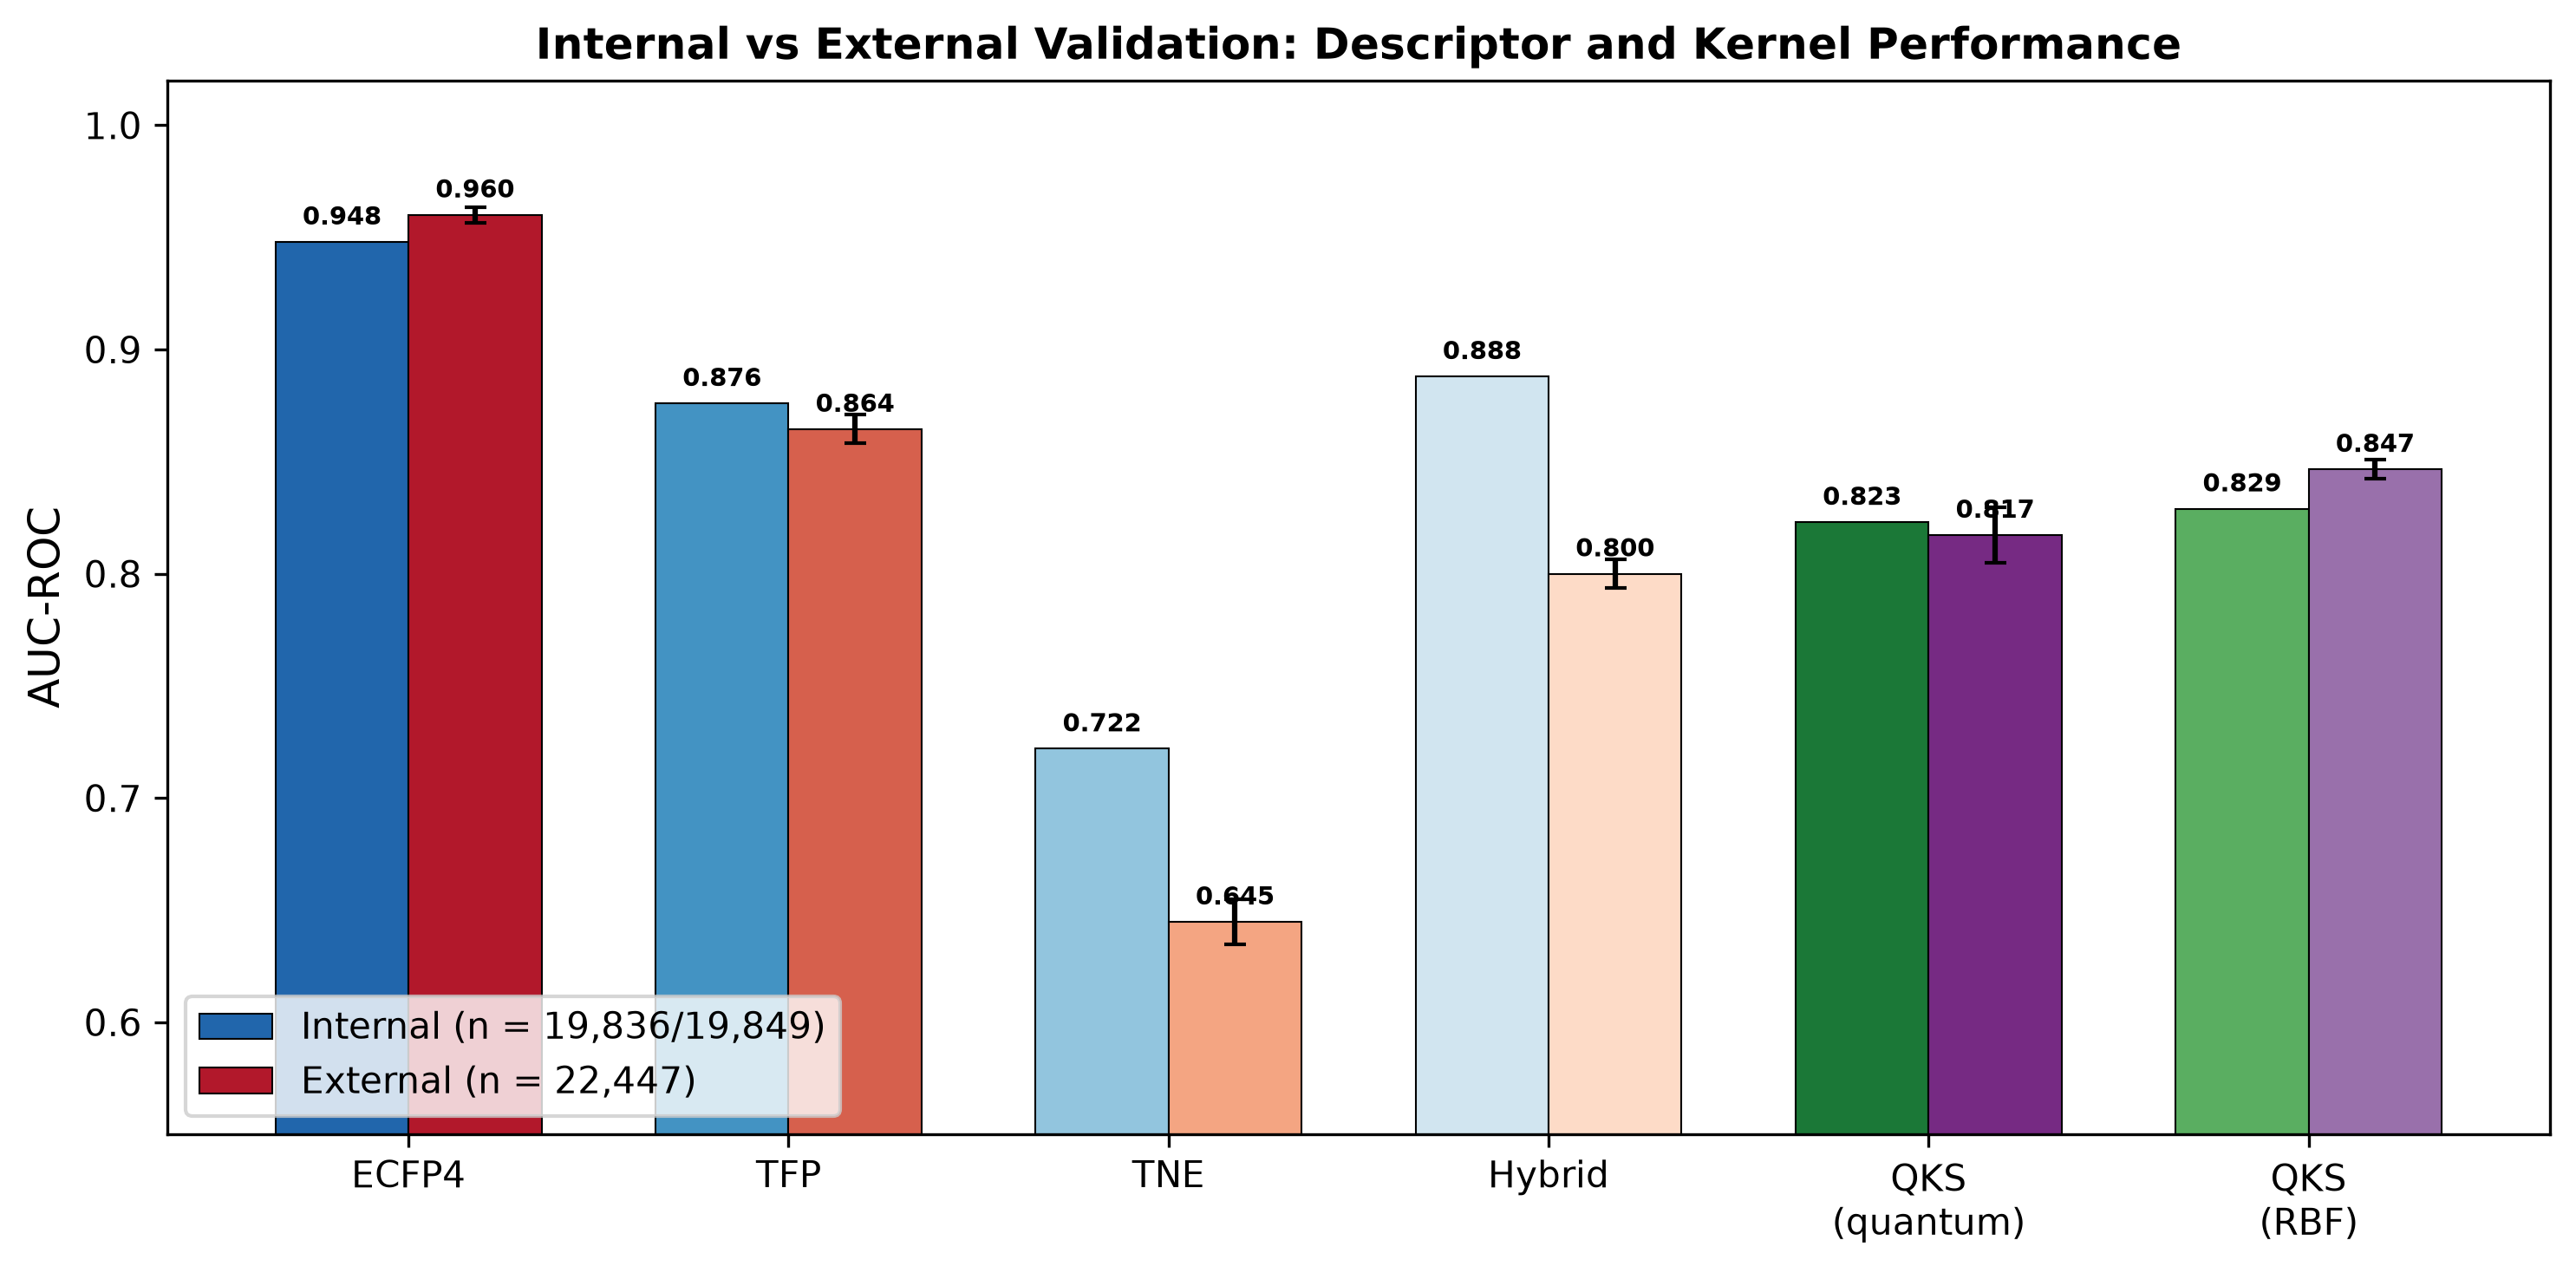
\includegraphics[width=0.85\textwidth]{p3_extval_internal_vs_external.png}
\caption{Internal versus external validation performance. Descriptor methods were evaluated with Random Forest; kernel methods with SVM. Error bars: standard deviation across 5 folds. External panel: ChEMBL antimalarial dataset ($n = \num{22447}$).}
\label{fig:extval_comparison}
\end{figure}

\subsection{Topological features correlate with binding promiscuity}

Across $N = \num{17011}$ molecules with multi-target docking data, H$_0$ count ($\rho = -\num{0.248}$, $p < 10^{-137}$), H$_0$ entropy ($\rho = -\num{0.243}$), and H$_1$ entropy ($\rho = -\num{0.190}$) negatively correlate with the number of targets bound ($\geq 2$ targets at $\Delta G \leq -\SI{7.0}{\kcalmol}$). Lower topological complexity thus associates with broader polypharmacological activity, consistent with reduced steric clash across multiple binding sites. The association between H$_1$ count and resistance-resilience scores is examined in the Supplementary Material (\cref{X-sec:tda_rrs}); after controlling for molecular size and structural covariates, the association is size-mediated and does not support an independent topological predictor.

% ============================================================================
% 4. DISCUSSION
% ============================================================================

\section{Discussion}

\subsection{Persistent homology as a diagnostic for generative-model evaluation}

The apparent contradiction between \qty{92.6}{\percent} Tanimoto distinction and \qty{69.3}{\percent} scaffold recovery arises because STONED-SELFIES mutations permute side-chains and functional groups (diverging H$_0$ connectivity) while preserving cyclic macro-structures (conserving H$_1$ ring topology). This decomposition has practical implications for generative-model evaluation: scaffold-only Tanimoto (\num{0.379}) is \num{1.84}$\times$ higher than whole-molecule Tanimoto (\num{0.206}), confirming that H$_1$ persistence diagrams capture scaffold identity independently of atom-level similarity. TFP provides an interpretable diagnostic for assessing whether molecular generation protocols preserve the ring systems essential for bioactivity---a capability absent from standard fingerprint-based diversity metrics.

\subsection{Tensor network compression: when low-rank structure helps}

Tucker decomposition exploits the fact that molecular tensors are approximately low-rank: the \num{6.1}$\times$ compression retains sufficient information for PfDHFR docking-score prediction ($R^2 = \num{0.473}$, competitive with ECFP4's \num{0.461}) while providing a fixed-length, physically interpretable embedding. The compression is not uniform across chemical space: molecules with common ring systems compress better (reconstruction error \num{0.098}) than structurally atypical molecules (\num{0.137}), and the atom-coordinate factor matrix correlates with molecular volume ($\rho = \num{0.71}$). This selective compression---preserving scaffold-relevant information while discarding noise---accounts for the higher chemical coherence of TNE clusters (Silhouette \num{0.35}) compared with ECFP4 (\num{0.18}) or VAE latent vectors (\num{0.229}), a property relevant for virtual screening where enrichment metrics depend on hit-cluster homogeneity.

\subsection{Kernel calibration, not quantum-ness, governs performance}

The central finding is that, with a properly tuned RBF baseline and the canonical 6-qubit circuit, the quantum kernel shows no statistically significant difference from the RBF kernel (internal: $p = \num{0.060}$ at $n = \num{19849}$; external: $p = \num{0.005}$ at $n = \num{22447}$). The external validation reveals a transfer gap that the internal comparison was underpowered to detect. This aligns with recent matched-baseline audits: QBioFusion-QSAR \citep{qbiofusion_2026} found quantum multiple-kernel learning improved small-data classification only for individual molecules, with no mean MCC gain, and parameter-matched comparisons \citep{iso_qgnn_2026} attribute topology-aligned architecture gains to inductive bias rather than quantum-ness.

Kernel choice and calibration matter more than the kernel's origin. For practitioners: (i)~always tune the RBF gamma by inner cross-validation before claiming quantum advantage; (ii)~the quantum kernel's $O(N^2)$ scaling restricts it to lead-optimisation sets of $\leq \num{10000}$ compounds; and (iii)~for primary virtual screening, ECFP4 (AUC \num{0.948}) remains the recommended baseline, with TFP and TNE as complementary descriptors for specific chemical-space regions.

\subsection{Distribution shift exposes tensor network fragility}

The \num{0.077} AUC degradation of TNE from internal (\num{0.722}) to external (\num{0.645}) validation is the largest among all descriptors and reflects Tucker decomposition's sensitivity to distribution shift. The \num{351} embedding failures (\num{1.6}\%) were concentrated in structurally complex natural products with unusual bond topologies---the chemical-space region where TNE compression is most needed but least reliable. Tensor-network descriptors should therefore be validated on external panels before deployment, and embedding failures should be reported transparently. TFP transferred well ($\Delta = -\num{0.011}$), indicating that persistent homology summary statistics are more robust to distribution shift than tensor core elements.

\subsection{Limitations}

Five limitations constrain interpretation. First, TFP does not outperform ECFP4 in activity prediction; it adds value primarily at the high-complexity tail (molecules with $\geq 3$ fused rings or $\geq 2$ stereocentres). Second, activity labels are computational predictions from Ersilia ML models, so all claims regarding activity and polypharmacology are predictions pending experimental validation. Third, the quantum kernel was evaluated on a classical simulator; NISQ hardware would degrade fidelity \citep{preskill2018nisq}. Fourth, we benchmarked against classical fingerprints but not against graph neural networks; our companion study \citep{temgoua2027gnn} evaluated GIN, GIN-TFP, GIN-TNE, and ChemBERTa on the same canonical panel and found that ECFP4-RF (scaffold AUC \num{0.8300}) outperformed all GNN architectures (best: GIN-TFP \num{0.8138}), confirming that for this dataset the classical fingerprint baseline is difficult to surpass regardless of model architecture. Fifth, the TNE component degrades on external data (\num{0.077} AUC loss), limiting its utility for cross-dataset transfer.

\subsection{Practical recommendations}

Based on these results and the companion GNN benchmark \citep{temgoua2027gnn}, we recommend: (i)~ECFP4-RF for virtual screening of African natural product libraries (AUC \num{0.948}, robust to distribution shift, outperforming GIN architectures on the same panel); (ii)~TFP for assessing scaffold preservation in generative campaigns (interpretable H$_1$/H$_0$ decomposition); (iii)~TNE only when fixed-length embeddings are required and external validation confirms reliability; and (iv)~QKS for retrospective mechanistic analysis on small lead-optimisation sets ($\leq \num{10000}$ compounds). Future work should integrate TDA features as node attributes in GNN architectures \citep{topologynet_2018}, validate descriptors experimentally, and explore whether topological features improve generalisation across therapeutic targets.

% ============================================================================
% 5. CONCLUSION
% ============================================================================

\section{Conclusion}

We introduced three molecular descriptors---persistent homology TFP, Tucker-compressed TNE, and simulated QKS---and benchmarked them on \num{19836} African antimalarial candidates. TFP resolves the scaffold paradox by decomposing molecular topology into conserved H$_1$ ring features and divergent H$_0$ connectivity. TNE achieves \num{6.1}$\times$ compression while retaining binding-relevant information competitive with ECFP4 for specific targets. The quantum kernel shows no significant advantage over a tuned RBF baseline; external validation reveals a transfer gap. These representations are complementary diagnostic tools that reveal topological dimensions of molecular structure, with ECFP4 remaining the recommended primary descriptor. Persistent homology decomposition provides an interpretable framework for evaluating generative-model outputs in natural product drug discovery.

% ============================================================================
% ACKNOWLEDGMENTS
% ============================================================================

\section*{Data Availability}

All data supporting the conclusions of this study are available in the public project repository at \url{https://github.com/NanaEngo/Malaria_codesV2} under the MIT licence. The Zenodo DOI \url{https://doi.org/10.5281/zenodo.19608875} is reserved, but the upload is pending and must not be treated as an existing archive. The deposit includes: (1)~TFP feature matrices for all \num{19849} library molecules; (2)~TNE embeddings (\num{192}-element Tucker core descriptors, bond dimension~8); (3)~quantum kernel matrices (6-qubit IQPEmbedding, PennyLane 0.45.1); (4)~all benchmark CSV files; (5)~the cross-paper H$_1$/RRS analysis dataset; and (6)~all analysis scripts.

\section*{List of Abbreviations}

\textbf{TFP:} topological fingerprint; \textbf{TNE:} tensor network embedding; \textbf{QKS:} quantum kernel score; \textbf{ECFP4:} extended-connectivity fingerprint, radius 2; \textbf{AP:} atom-pair fingerprint; \textbf{BPF:} binding-pattern fingerprint; \textbf{FCFP4:} functional-class fingerprint, radius 2; \textbf{MACCS:} MACCS structural keys; \textbf{PHCO:} pharmacophore fingerprint; \textbf{H$_0$/H$_1$/H$_2$:} 0th/1st/2nd persistent homology dimensions; \textbf{AUC:} area under the receiver operating characteristic curve; \textbf{RBF:} radial basis function; \textbf{RRS:} resistance resilience score; \textbf{NISQ:} noisy intermediate-scale quantum; \textbf{UMAP:} uniform manifold approximation and projection; \textbf{RF:} random forest; \textbf{SVM:} support vector machine.

\section*{Acknowledgments}

We thank the developers of Ripser, TensorLy, and PennyLane for open-source software. Computational resources were provided by the University of Yaound\'{e}~I HPC facility.

\section*{Authors' Contributions}

Myke Vital Sao Temgoua: conceptualization, methodology, software, formal analysis, investigation, data curation, writing -- original draft. Jean-Pierre Tchapet Njafa: conceptualization, methodology, software, supervision, writing -- review \& editing. Serge Guy Nana Engo: methodology, supervision, writing -- review \& editing. Penabei Samafou: data curation, writing -- review \& editing. Wilfred Fon Mbacham: conceptualization, validation, writing -- review \& editing. All authors read and approved the final manuscript.

\section*{Funding}

This research received no specific grant from any funding agency in the public, commercial, or not-for-profit sectors.

\section*{Ethics approval and consent to participate}

Not applicable. This study is entirely computational and uses publicly available chemical databases and in-silico activity predictions; no human or animal subjects or patient data were involved.

\section*{Consent for publication}

Not applicable. No individual person's data appear in this manuscript.

\section*{Competing Interests}

The authors declare no competing interests.

\section*{Use of Artificial Intelligence}

During the preparation of this work the authors used AI assistants to support code development and data analysis scripting. The authors reviewed and edited all AI-assisted output and take full responsibility for the content of this article. No generative AI tool is listed as an author.

% ============================================================================
% BIBLIOGRAPHY
% ============================================================================

\bibliographystyle{unsrtnat}
\bibliography{Bibliography_Paper3}

\end{document}
